\begin{figure}
    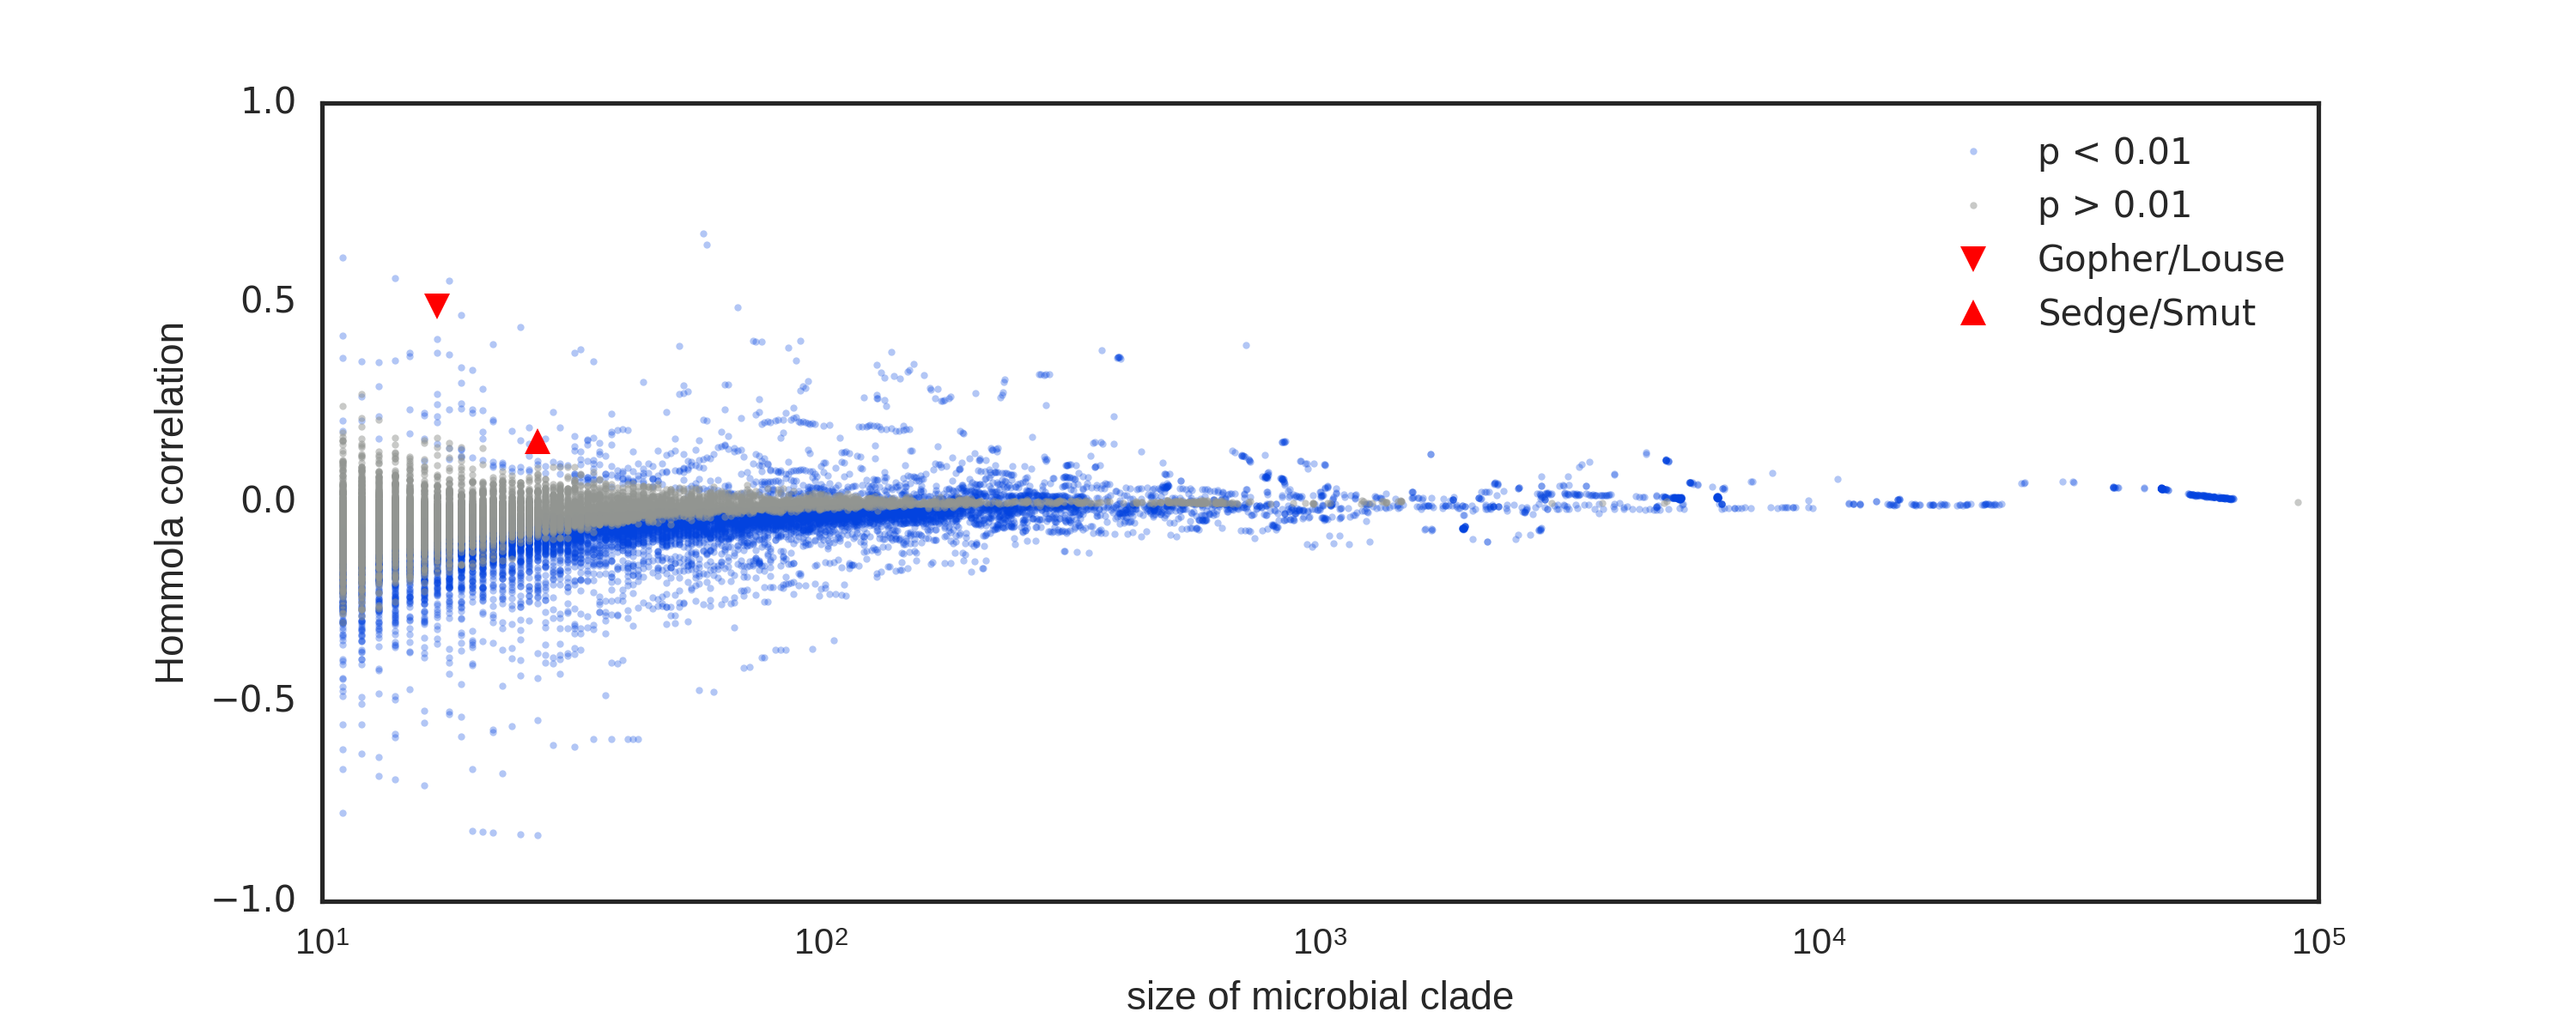
\includegraphics[width=\textwidth]{FishPoo/figures/Hommola_correlations.png}
    \caption{The Hommola correlation coefficient of the 70,343 host-associated microbial clades with more than five members. The average clade contains 228 host-associated OTUs, and the largest contains 90,858 OTUs. Statistically significant correlations (those with $p$ values less than 0.01) are shown in blue, and non-significant correlations are shown in gray. For comparison, two reference case are included; the pocket gopher and chewing louse system from Hafner {\em et al.} ($r=0.49$, $p=1.38\times 10^{-9}$, 17 host-associated taxa) and the sedge grasses and smut fungi system from Escudero ($r=0.15$, $p=1.27\times 10^{-5}$, 27 host-associated taxa). \cite{hafner1994disparate,escudero2015phylogenetic} Of thse, 343 clades show statistically significant Hommola correlations exceeding 0.1.}
    \label{FP_hommola_corr}
\end{figure}
